%
% phdtex
%
% Copyright (c) 2014-2020, Andrew Kanner <andrew.kanner@gmail.com>.
% All rights reserved.
%
% SPDX-License-Identifier: MIT
%

\documentclass[a5paper,10pt]{report}
% добавить leqno в [] для нумерации объектов слева
%\documentclass[a5paper,10pt,twoside]{report}

\IfFileExists{./template/contrib/styles.tex}{\def\template{./template}}{\def\template{.}}

% подключаемые пакеты, стили (в т.ч. ГОСТ Р 7.0.11-2011)
%%% Поля и разметка страницы %%%
\usepackage{lscape}		% Для включения альбомных страниц
\usepackage{geometry}	% Для последующего задания полей

%%% Кодировки и шрифты %%%
\usepackage{cmap}						% Улучшенный поиск русских слов в полученном pdf-файле
\usepackage[T2A]{fontenc}				% Поддержка русских букв (кодировка)
\usepackage[utf8]{inputenc}				% Кодировка utf8 (исходного текста)
\usepackage[english, russian]{babel}	% Языки: русский, английский (локализация и переносы)
\usepackage{pscyr}						% Красивые русские шрифты
\usepackage{extsizes}					% Возможность сделать 14-й шрифт

%%% Альтернативные шрифты %%%
%\usepackage[english, russian]{babel}
%\usepackage{fontspec}					% загрузка шрифтов Open Type, True Type и др.
%\usepackage{euscript}					% Шрифт Евклид
%\usepackage{mathrsfs}					% Красивый матшрифт

%%% Оформление абзацев, колонтитулов, текста %%%
\usepackage{indentfirst}	% Красная строка
\frenchspacing
\usepackage{fancyhdr}		% Колонтитулы
\usepackage{setspace}		% Интерлиньяж

%%% Математические пакеты %%%
\usepackage{amsmath,amsfonts,amssymb,amsthm,mathtools,amscd}	% Математические дополнения от AMS
\usepackage{icomma}												% "Умная" запятая: $0,2$ --- число, $0, 2$ --- перечисление
\usepackage{mathtext}											% русские буквы в формулах
%\usepackage{leqno}												% Нумерация формул слева

%%% Цвета %%%
\usepackage[usenames]{color}
\usepackage{color}
\usepackage{colortbl}
\usepackage[usenames,dvipsnames,svgnames,table,rgb]{xcolor}

%%% Таблицы %%%
\usepackage{array,tabularx,tabulary,booktabs}	% Дополнительная работа с таблицами
\usepackage{longtable}							% Длинные таблицы
\usepackage{multirow,makecell}					% Улучшенное форматирование таблиц (слияние строк и т.п.)

%%% Общее форматирование
\usepackage[singlelinecheck=off,center]{caption}	% Многострочные подписи
\usepackage{soul}									% Поддержка переносоустойчивых подчёркиваний и зачёркиваний
%\usepackage{soulutf8}								% Аналогичные модификаторы начертания

%%% Библиография %%%
\usepackage{cite}				% Красивые ссылки на литературу (библиография)
%\usepackage[superscript]{cite}	% Ссылки в верхних индексах
%\usepackage[nocompress]{cite}
\usepackage{csquotes}			% Еще инструменты для ссылок
%\usepackage[backend=biber,bibencoding=utf8,sorting=ynt,maxcitenames=2,style=authoryear]{biblatex}
%\addbibresource{bib1.bib}
%\usepackage[style=authoryear,maxcitenames=2,backend=biber,sorting=nty]{biblatex}

%%% Гиперссылки %%%
\usepackage[linktocpage=true,plainpages=false,pdfpagelabels=false]{hyperref}

%%% Изображения %%%
\usepackage{graphicx}	% Подключаем пакет работы с графикой
\usepackage{wrapfig}	% Обтекание рисунков текстом

%%% Оглавление %%%
\usepackage{tocloft}

%%% Программирование %%%
\usepackage{etoolbox}	% логические операторы

%%% Рисование
\usepackage{tikz}		% Работа с графикой
\usepackage{pgfplots}
\usepackage{pgfplotstable}

%%% Другие пакеты %%%
\usepackage{lastpage}	% Узнать, сколько всего страниц в документе.
\usepackage{multicol}	% Несколько колонок
\usepackage{totcount}	% Счетчики для глав, приложений и т.д.

%
% phdtex
%
% Copyright (c) 2014-2017, Andrew Kanner <andrew.kanner@gmail.com>.
% All rights reserved.
%
% SPDX-License-Identifier: MIT
%

%% Макет страницы, поля и разметка [перенесено в stylesgost.tex]
%\geometry{a4paper,top=2cm,bottom=2cm,left=3cm,right=1cm}

%% Кодировки и шрифты
% times new roman
\renewcommand{\rmdefault}{ftm}

%% Альтернативные шрифты (см. packages.tex)
% свойства шрифтов по умолчанию
%\defaultfontfeatures{Ligatures={TeX},Renderer=Basic}
% основной шрифт документа
%\setmainfont[Ligatures={TeX,Historic}]{Times New Roman}
% шрифт без засечек
%\setsansfont{Comic Sans MS}
%\setmonofont{Courier New}
% начертание шрифта
%\renewcommand{\familydefault}{\sfdefault}

%% Номера формул
% номера только у тех формул, на которые есть \eqref{} в тексте
%\mathtoolsset{showonlyrefs=true}

%% Выравнивание и переносы
% не допускать переполнений
\sloppy
% запретить разрыв страницы после первой строки абзаца
\clubpenalty=10000
% запретить разрыв страницы после последней строки абзаца
\widowpenalty=10000
% для растягивания или игнорирования "Underfull \hbox"
%\setlength{\emergencystretch}{1pt}
%\sloppy
% глобальные правила переноса (или запрета переноса)
%\hyphenation{сло-во}
% "Overfull", стандартный допустимый: 0.1pt
%\hfuzz=2.5pt
% разреженность, стандартный порог: 200
%\tolerance=400

% кастомные стили для теорем, утверждений и прочего
\newtheoremstyle{plain-indent} % name
{\topsep} % Space above
{\topsep} % Space below
{\itshape} % Body font
%{0pt} % Indent amount
{\parindent} % [New] indent to match GOST
{\bfseries} % Theorem head font
{.} % Punctuation after theorem head
{5pt plus 1pt minus 1pt} % Space after theorem head
{} % Theorem head spec

\newtheoremstyle{definition-indent}
{\topsep}
{\topsep}
{\normalfont} % diff
%{0pt}
{\parindent}
{\bfseries}
{.}
{5pt plus 1pt minus 1pt}
{}

\newtheoremstyle{remark-indent}
{0.5\topsep} % diff
{0.5\topsep} % diff
{\normalfont} % diff
%{0pt}
{\parindent}
{\itshape} % diff
{.}
{5pt plus 1pt minus 1pt}
{}

%% Математические конструкции (теоремы, утверждения и т.д.)
% стиль по умолчанию
\theoremstyle{plain-indent}
\newtheorem{theorem}{Теорема}
\newtheorem{proposition}{Утверждение}
\newtheorem{lemma}{Лемма}
% стиль определений
\theoremstyle{definition-indent}
\newtheorem{corollary}{Следствие}
\newtheorem{problem}{Задача}[section]
\newtheorem{condition}{Условие}
\newtheorem{definition}{Определение}
\newtheorem{axiom}{Аксиома}
% стиль примечаний
\theoremstyle{remark-indent}
\newtheorem*{nonum}{Решение}

%% Цветовые эффекты (выделение текста)
\newcommand\hly[1]{\colorbox{yellow!80}{\begin{varwidth}{\dimexpr\linewidth-2\fboxsep}#1\end{varwidth}}}
\newcommand\hlg[1]{\colorbox{green!80}{\begin{varwidth}{\dimexpr\linewidth-2\fboxsep}#1\end{varwidth}}}
% цветные текст-боксы для таблиц и графиков
\newcommand\hlyy[1]{\fcolorbox{black!50}{yellow!25}{\begin{varwidth}{\dimexpr\linewidth-2\fboxsep}#1\end{varwidth}}}
\newcommand\hlgg[1]{\fcolorbox{black!50}{green!25}{\begin{varwidth}{\dimexpr\linewidth-2\fboxsep}#1\end{varwidth}}}
\newcommand\hlbrr[1]{\fcolorbox{black!50}{brown!25}{\begin{varwidth}{\dimexpr\linewidth-2\fboxsep}#1\end{varwidth}}}
\newcommand\hlbll[1]{\fcolorbox{black!50}{black!25}{\begin{varwidth}{\dimexpr\linewidth-2\fboxsep}#1\end{varwidth}}}
\newcommand\hlrr[1]{\fcolorbox{black!50}{red!25}{\begin{varwidth}{\dimexpr\linewidth-2\fboxsep}#1\end{varwidth}}}
\newcommand\hlbluu[1]{\fcolorbox{black!50}{blue!25}{\begin{varwidth}{\dimexpr\linewidth-2\fboxsep}#1\end{varwidth}}}
\newcommand\hlempty[1]{\fcolorbox{black!50}{white}{\begin{varwidth}{\dimexpr\linewidth-2\fboxsep}#1\end{varwidth}}}
\newcommand\hlbr[1]{\colorbox{brown!80}{\begin{varwidth}{\dimexpr\linewidth-2\fboxsep}#1\end{varwidth}}}
\newcommand\hlbl[1]{\colorbox{black!80}{\begin{varwidth}{\dimexpr\linewidth-2\fboxsep}#1\end{varwidth}}}
\newcommand\hlr[1]{\colorbox{red!80}{\begin{varwidth}{\dimexpr\linewidth-2\fboxsep}#1\end{varwidth}}}
\newcommand\hlblu[1]{\colorbox{blue!80}{\begin{varwidth}{\dimexpr\linewidth-2\fboxsep}#1\end{varwidth}}}
% deprecated вариант2
% \newcommand\hl{\bgroup\markoverwith{\textcolor{yellow}{\rule[-.5ex]{2pt}{2.5ex}}}\ULon}
% deprecated вариант3
%\newcommand*{\hl}[1]{\colorbox{yellow}{#1}}

%% Изображения
% путь к каталогу с изображениями
\graphicspath{{images/}}
% отступ рамки \fbox{} от рисунка
\setlength\fboxsep{3pt}
% толщина линий рамки \fbox{}
\setlength\fboxrule{1pt}

%% Библиография
\makeatletter
% библиография в соответствии с ГОСТ 7.1-2003
\bibliographystyle{\template/contrib/utf8gost71my}
% заменить квадратные скобки на точку
\renewcommand{\@biblabel}[1]{#1.}
\makeatother

%% Гиперссылки: цвета и другие настройки
\definecolor{linkcolor}{rgb}{0.9,0,0}
\definecolor{citecolor}{rgb}{0,0.6,0}
\definecolor{urlcolor}{rgb}{0,0,1}
\hypersetup{
  % русские буквы в разделах
  unicode=true,
  % true: цветные ссылки; false: ссылки в рамках
  colorlinks=true,
  % внутренние ссылки
  linkcolor={linkcolor},
  % ссылки на библиографию
  citecolor={citecolor},
  % на файлы
  filecolor=magenta,
  % на URL
  urlcolor={urlcolor}
}

%% Оглавление
\renewcommand{\cftchapdotsep}{\cftdotsep}


%% Листинги
% стиль javascript
\lstdefinelanguage{JavaScript}{
  keywords={break, case, catch, continue, debugger, default, delete,
    do, else, false, finally, for, function, if, in, instanceof, new,
    null, return, switch, this, throw, true, try, typeof, var, void,
    while, with},
  comment=[l]{//},
  morecomment=[s]{/*}{*/},
  morestring=[b]',
  morestring=[b]",
  ndkeywords={class, export, boolean, throw, implements, import,
    this},
  keywordstyle=\color{blue}\bfseries,
  ndkeywordstyle=\color{yellow}\bfseries,
  identifierstyle=\color{black},
  commentstyle=\color{green}\ttfamily,
  stringstyle=\color{red}\ttfamily
  sensitive=true,
}
% стиль xml
\lstdefinelanguage{xml}{
  morekeywords={name,description,memory,unit,os,arch,machine,devices,emulator,hostdev,
    mode, type, managed, source, vendor, id, product, address, domain,
    bus, slot, function},
  numbers=none,
  frame=none,
  belowskip=2pt,
  caption=,
}
% стиль bash
\lstdefinelanguage{bashhh}{
  morekeywords={modprobe,echo},
  deletekeywords={bind},
  morecomment=[l]{\#},
  numbers=none,
  frame=none,
  belowskip=2pt,
  caption=,
}
% цветовая схема для выделения блоков кода
\definecolor{codegreen}{rgb}{0,0.6,0}
\definecolor{codegray}{rgb}{0.5,0.5,0.5}
\definecolor{codemauve}{rgb}{0.58,0,0.82}
\lstset{
  % язык программирования [должен выставляться в самом листинге!]
  % language=C,
  % language=JavaScript,
  % моноширинный шрифт
  columns=fixed,
  % цвет фона (использует пакеты color/xcolor)
  backgroundcolor=\color{white},
  % размер и начертание
  basicstyle=\small\sffamily,
  % перенос строки только при наличии пробела
  breakatwhitespace=false,
  % автоматический перенос строк
  breaklines=true,
  % позиция заголовка (вверху: t, внизу: b)
  captionpos=b,
  % стиль для комментариев
  commentstyle=\color{codegreen},
  % стиль для ключевых слов
  keywordstyle=\color{blue},
  % дополнительные ключевые слова
  morekeywords={*,...},
  % можно удалить какие-нибудь ключевые слова
  deletekeywords={...},
  % для использования latex в коде
  escapeinside={\%*}{*)},
  % разрешить использовать не-ASCII символы
  extendedchars=true,
  % extendedchars=\true,
  % inputencoding=utf8x,
  % keepspaces = true,
  % добавить рамку вокруг кода
  frame=single,
  % если не установлено, то цвет рамки может меняться
  rulecolor=\color{black},
  % позиция номеров строк
  numbers=left,
  % расстояние от номера строки до кода
  numbersep=5pt,
  % размер шага между номерами строк
  stepnumber=1,
  % стиль для номеров строк
  numberstyle=\tiny\color{codegray},
  % не показывать пробелы в виде отступов
  showspaces=false,
  % не показывать пробелы в строках
  showstringspaces=false,
  % не показывать знаки табуляции
  showtabs=false,
  % стиль для строковых литералов
  stringstyle=\color{codemauve},
  % размер табуляции
  tabsize=2,
  % показывать имя подключаемого файла
  title=\lstname
}

%% Разное
% использовать \slash для переноса слов, разделенных "\"?

%%% Колонтитулы (см. packages.tex) %%%
\pagestyle{fancy}
\renewcommand{\headrulewidth}{0pt}	% Толщина линейки, отчеркивающей верхний колонтитул
%\lfoot{Нижний левый}
%\rfoot{Нижний правый}
%\rhead{Верхний правый}
%\chead{Верхний в центре}
%\lhead{Верхний левый}
%\cfoot{Нижний в центре}			% По умолчанию здесь номер страницы
\lfoot{}
\rfoot{}
\rhead{}
\chead{\normalsize\thepage}
\lhead{}
\cfoot{}

%%% при использовании chapters - первая страница создается в plain pagestyle %%%
\fancypagestyle{plain}{\pagestyle{fancy}}

%%% Интерлиньяж %%%
\onehalfspacing	% Интерлиньяж 1.5
%\doublespacing	% Интерлиньяж 2
%\singlespacing	% Интерлиньяж 1

%%% Макет страницы %%%
\geometry{a4paper,top=20mm,bottom=20mm,left=25mm,right=10mm}

\usepackage{sectsty}
\allsectionsfont{\centering}	% центрирование заголовков (должны быть без точки на конце и переносов)

%%% список сокращений %%%
\usepackage{nomencl}

% Позволяет одновременно печатать условное обозначение в тексте документа и добавлять его в перечень
\newcommand*{\nom}[2]{#1\nomenclature{#1}{#2}}

%%% Формат формул и ссылок на формулы %%%
% ПРИМЕР:
%\begin{equation}\label{name}
%	2+2=4
%\end{equation}
%
%Формула \eqref{name}

% Перечень сокращений будет распечатываться по алфавиту вне зависимости от появления в тексте
% ПРИМЕР:
%\nom{Б}{Вторая буква алфавита}.
%А\nomenclature{А}{Первая буква алфавита}

% Список литературы формируется в порядке возрастания - bib1, bib2, bib3,...
% по ГОСТ НЕОБХОДИМО, чтобы источники на отличном от русского языке перечислялись ПОСЛЕ источников на русском

% Приложения ДОЛЖНЫ быть перечислены в порядке их перечисления в тексте

% добавим файл с информацией по работе, автору и т.д.
% !TEX root = dissertation.tex synopsis.tex

%
% phdtex
%
% Copyright (c) 2014-2020, Andrew Kanner <andrew.kanner@gmail.com>.
% All rights reserved.
%
% SPDX-License-Identifier: CC-BY-4.0
%

% заголовок
\author{ФАМИЛИЯ ИМЯ ОТЧЕСТВО автора}
\title{НАЗВАНИЕ ДИССЕРТАЦИОННОЙ РАБОТЫ}

% неизменяемые общие данные
\date{\today}
\makeatletter
\def\dissauthor{\@author}
\def\disstitle{\@title}
\def\dissdate{\@date}
\makeatother
\def\dissyear{\the\year}

% специальность, ученая степень, руководитель, консультант, оппоненты
\def\specnum{ХХ.ХХ.ХХ}
\def\specname{<<Название специальности>>}
\def\edudegree{кандидата каких-то там наук}
\def\mentordegree{уч. степень, уч. звание}
%\def\mentortitle{уч. звание}
\def\mentorcompany{Название\\компании,\\г. Город\\~}
\def\mentorname{Фамилия И. О.}
\def\consultantdegree{уч. степень}
\def\consultantcompany{Название компании,\\ г. Город}
\def\consultantname{Фамилия И. О.}
\def\opponentonedegree{уч. степень}
\def\opponentonecompany{\\Название компании,\\ г. Город}
\def\opponentonename{Фамилия И. О.}
\def\opponenttwodegree{уч. степень}
\def\opponenttwocompany{\\Название компании,\\ г. Город}
\def\opponenttwoname{Фамилия И. О.}
\def\opponentthreedegree{уч. степень}
\def\opponentthreecompany{\\Название компании,\\ г. Город}
\def\opponentthreename{Фамилия И. О.}
\def\leadingorg{Название ведущей организации}

% прочие данные
\def\disscity{Город }
\def\dissorg{НАЗВАНИЕ УЧРЕЖДЕНИЯ, В КОТОРОМ ВЫПОЛНЯЛАСЬ\par
ДАННАЯ ДИССЕРТАЦИОННАЯ РАБОТА\par}
\def\dissorgsyn{<<Название учреждения, в котором выполнялась данная
  диссертационная работа>>}
\def\dissudk{УДК xxx.xxx}

% данные для оборота титульного листа автореферата
\def\councildate{<<\dots>> \dots \the\year~г.}
\def\counciltime{\dots:00}
\def\councilnum{Д xxx.xxx.xx}
\def\councilplace{<<Организация, к которой относится диссертационный
  совет>>}
\def\counciladdress{Индекс, г.~Город, шоссе / улица / \dots,~д.xx}
\def\libraryname{<<Организация, куда передается рукопись
  диссертационной работы>> и на сайте:}
\def\libraryaddress{Индекс, г.~Город, шоссе / улица / \dots,~д.xx}
\def\councilwebsite{http://website.ru}
\def\synopsissentdate{<<\dots>> \dots \the\year~года}
\def\councilsecretarydegree{уч. степень, уч. звание}
\def\councilsecretaryname{И.О.~Фамилия}

% выставим атрибуты pdf-документа
\hypersetup{
  % заголовок
  pdftitle={\disstitle},
  % автор
  pdfauthor={\dissauthor},
  % тема
  pdfsubject={\disstitle},
  % создатель
  pdfcreator={\dissauthor},
  % производитель
  pdfproducer={\dissauthor},
  % ключевые слова
  pdfkeywords={keyword1} {keyword2}
}


% \includeonly{\template/synopsis-parts/synopsis-title,
% parts/intro-syn, synopsis-parts/synopsis-content,
% synopsis-parts/synopsis-results}

% для использования ссылок на страницы текста диссертации
\usepackage{refcount,xr}
\externaldocument{\template/parts/lists}
\externaldocument{parts/appendix}

% раздельная библиография в автореферате [переопределяет styles.tex!]
\usepackage{bibtopic}
\bibliographystyle{\template/contrib/utf8gost71my-unsort}

% другой размер бумаги для автореферата (A5)
\geometry{a5paper,top=15mm,bottom=20mm,left=15mm,right=12mm}

% номер страницы в автореферате снизу
\chead{}
\cfoot{\normalsize\thepage}

% сделаем нежирные заголовки в автореферате
\allsectionsfont{\normalfont\centering\raggedright}

% другой формат подразделов автореферата
\titleformat*{\subsection}{\centering\normalsize}

\begin{document}

% переопределение именований
%
% phdtex
%
% Copyright (c) 2014-2017, Andrew Kanner <andrew.kanner@gmail.com>.
% All rights reserved.
%
% SPDX-License-Identifier: MIT
%

% переопределение именований
\renewcommand{\abstractname}{Аннотация}
\renewcommand{\alsoname}{см. также}
\renewcommand{\appendixname}{Приложение}
\renewcommand{\bibname}{Список использованных источников}
\renewcommand{\ccname}{исх.}
\renewcommand{\chaptername}{Глава}
\renewcommand{\contentsname}{Содержание}
\renewcommand{\enclname}{вкл.}
\renewcommand{\figurename}{Рисунок}
\renewcommand{\headtoname}{вх.}
\renewcommand{\indexname}{Предметный указатель}
\renewcommand{\listfigurename}{Список рисунков}
\renewcommand{\listtablename}{Список таблиц}
\renewcommand{\pagename}{Стр.}
\renewcommand{\partname}{Часть}
\renewcommand{\refname}{Список литературы}
\renewcommand{\seename}{см.}
\renewcommand{\tablename}{Таблица}
\renewcommand{\lstlistingname}{Листинг}

% заголовок перечня nomenclature
\renewcommand{\nomname}{Перечень сокращений и условных обозначений}

% переопределение математических символов на русский манер
\renewcommand{\epsilon}{\ensuremath{\varepsilon}}
\renewcommand{\phi}{\ensuremath{\varphi}}
\renewcommand{\kappa}{\ensuremath{\varkappa}}
\renewcommand{\le}{\ensuremath{\leqslant}}
\renewcommand{\leq}{\ensuremath{\leqslant}}
\renewcommand{\ge}{\ensuremath{\geqslant}}
\renewcommand{\geq}{\ensuremath{\geqslant}}
\renewcommand{\emptyset}{\varnothing}

% перенос знаков в формулах (по Львовскому)
\newcommand*{\hm}[1]{#1\nobreak\discretionary{}
{\hbox{$\mathsurround=0pt #1$}}{}}

% сокращения
\newcommand*{\linux}{GNU/Linux}
\newcommand*{\linuxkernel}{Linux}

% дополнительные команды
%\DeclareMathOperator{\sgn}{\mathop{sgn}}
\newcommand*{\nbline}{\\*\indent}
\newcommand{\tab}[1]{\hspace{.1\textwidth}\rlap{#1}}
\newcommand*{\ti}[1]{\text{\textit{#1}}}

% счетчик для пунктов в первом столбце таблиц
\newcounter{rowcount}
\setcounter{rowcount}{0}
\newcommand\rownumber{\stepcounter{rowcount}\arabic{rowcount}.}


% титульный лист автореферата с оборотом
% !TEX root = ../synopsis.tex

%
% phdtex
%
% Copyright (c) 2014-2020, Andrew Kanner <andrew.kanner@gmail.com>.
% All rights reserved.
%
% SPDX-License-Identifier: MIT
%

\thispagestyle{empty}

\begin{center}
	\dissorg
	\par
\end{center}

\begin{flushright}
На правах рукописи

{\sl \dissudk}
\end{flushright}

\vspace{30mm}
\begin{center}
{\large \dissauthor}
\end{center}

\vspace{10mm}
\begin{center}
{\large \MakeUppercase{\disstitle}
\par}

\vspace{5mm}
{%\small
\specnum~---~\specname
}

\vspace{15mm}
\MakeUppercase{Автореферат}

диссертации на соискание ученой степени

\edudegree
\end{center}

\vspace{10mm}
Автор:

\vfill
\begin{center}
{\disscity -- \dissyear}
\end{center}



\newpage
%%% оборотная сторона
\thispagestyle{empty}
\noindent Диссертационная работа выполнена в \dissorgsyn.

\begin{table}[h]
	\begin{tabular}{@{}ll}

	% Научный руководитель -- 6 строк (ФИО, ученое звание, должность)
	\makecell[l]{Научный руководитель:\\~\\~\\~\\~\\~} &
		\makecell*[{{p{10cm}}}]{
			\textbf{\mentorname} \\ \mentordegree, \mentorcompany
		}\\
	%\vspace{1mm}

	% Научный консультант -- 3 строки
	\makecell[l]{Научный консультант:\\~\\~} &
		\makecell*[{{p{10cm}}}]{
			\textbf{\consultantname} \\ \consultantdegree, \consultantcompany
		}\\
	%\vspace{1mm}

	% Оппоненты -- по 4 строки
	\makecell[l]{Официальные оппоненты:\\~\\~\\~} &
		\makecell[{{p{10cm}}}]{
			\textbf{\opponentonename} \\ \opponentonedegree, \opponentonecompany
		}\\
	\vspace{3mm}

	\makecell[l]{~\\~\\~\\~} &
		\makecell[{{p{10cm}}}]{
			\textbf{\opponenttwoname} \\ \opponenttwodegree, \opponenttwocompany
		}\\
%	\vspace{3mm}

	\makecell[l]{~\\~\\~\\~} &
		\makecell[{{p{10cm}}}]{
			\textbf{\opponentthreename} \\ \opponentthreedegree, \opponentthreecompany
		}

	%\vspace{3mm}
%	\makecell[l]{Ведущая организация:} &
%		\makecell*[{{p{11cm}}}]{\textbf{\leadingorg}}
  \end{tabular}
\end{table}

\noindent Защита состоится \councildate~в~\counciltime~часов
на~заседании диссертационного совета \councilnum{} при
\councilplace{} по адресу: \counciladdress.

\vspace{1mm}
\noindent С диссертацией можно ознакомиться в библиотеке
\libraryname{} и на сайте:
\councilwebsite{}. % по адресу: \libraryaddress.

\vspace{1mm}
\noindentАвтореферат разослан \synopsissentdate.

\vfill
\begin{table}[h]
  \begin{tabular}{@{}p{9.5cm}cr}
    \begin{tabular}{@{}p{8cm}}
      Ученый секретарь диссертационного совета \\	\councilnum,
      \councilsecretarydegree \\~
    \end{tabular} &
    % \begin{tabular}{@{}c}
    % 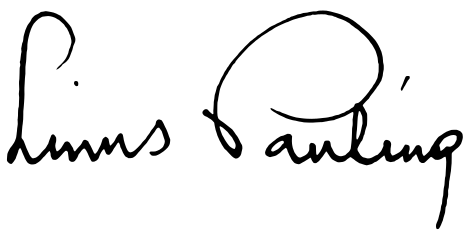
\includegraphics[height=2cm]{coucilsecretarysignature}
    % \end{tabular} &
                      \begin{tabular}{@{}r}
			\councilsecretaryname \\
                        \\
                        \\
                      \end{tabular}
  \end{tabular}
\end{table}

% \newpage

\resetHeadWidth

% текст введения находится в introduction.tex
% !TEX root = ../synopsis.tex

%
% phdtex
%
% Copyright (c) 2014-2017, Andrew Kanner <andrew.kanner@gmail.com>.
% All rights reserved.
%
% SPDX-License-Identifier: CC-BY-4.0
%

% вынесено из 02-introduction.tex с целью: 1. использования разных
% заголовков в автореферате и тексте диссертации 2. добавления в
% автореферат блока со структурой работы

% нумерация с 3й страницы
\setcounter{page}{3}

% заголовок
\subsection*{\MakeUppercase{Общая характеристика работы}}

% введение
% !TEX root = dissertation.tex

\chapter*{Введение}							% Заголовок
\addcontentsline{toc}{chapter}{Введение}	% Добавляем его в оглавление
Обзор, введение в тему, обозначение места данной работы в мировых исследованиях и т.п.

\textbf{Целью} данной работы является \ldots

Для~достижения поставленной цели необходимо было решить следующие задачи:
\begin{enumerate}
  \item Исследовать, разработать, вычислить и т.д. и т.п.
  \item Исследовать, разработать, вычислить и т.д. и т.п.
  \item Исследовать, разработать, вычислить и т.д. и т.п.
  \item Исследовать, разработать, вычислить и т.д. и т.п.
\end{enumerate}

\textbf{Основные положения, выносимые на~защиту:}
\begin{enumerate}
  \item Первое положение
  \item Второе положение
  \item Третье положение
  \item Четвертое положение
\end{enumerate}

\textbf{Научная новизна:}
\begin{enumerate}
  \item Впервые \ldots
  \item Впервые \ldots
  \item Было выполнено оригинальное исследование \ldots
\end{enumerate}

\textbf{Научная и практическая значимость} \ldots

\textbf{Степень достоверности} полученных результатов обеспечивается \ldots Результаты находятся в соответствии с результатами, полученными другими авторами.

\textbf{Апробация работы.}
Основные результаты работы докладывались~на:
перечисление основных конференций, симпозиумов и т.п.

\textbf{Личный вклад.} Автор принимал активное участие \ldots

\textbf{Публикации.} Основные результаты по теме диссертации изложены в ХХ печатных изданиях~\cite{bib1,bib2,bib3,bib4,bib5},
Х из которых изданы в журналах, рекомендованных ВАК~\cite{bib1,bib2,bib3}, 
ХХ --- в тезисах докладов~\cite{bib4,bib5}.

\textbf{Объем и структура работы.} Диссертация состоит из~введения, \total{chapnum} глав, заключения и~\total{appendnum} приложени\hly{я}. Полный объем диссертации составляет \pageref{LastPage}~страниц\hly{ы} с~\hly{ХХ}~рисунками и~\hly{ХХ}~таблицами. Количество наименований в списке литературы --- \total{bibnum}.

%\clearpage

% автоматически проставить значения переменных как в тексте
% диссертации тут нельзя -- обновлять нужно вручную (в тексте --
% \total{chapnum}, \total{appendnum}, \pageref{LastPage},
% \total{bibnum} и другие)
\underline{Структура и объем работы}. Диссертационная работа состоит
из~введения, \hly{X} глав, заключения и~\hly{X} приложений. Объем
основного текста диссертации составляет \hly{XXX}~страниц
с~\hly{XX}~рисунками и~\hly{XX}~таблицами. Приложение также содержит
документы, подтверждающие практическое использование и внедрение
результатов диссертационного исследования. Количество наименований в
списке литературы --- \hly{XXX}.

% содержание работы по главам, основные результаты и выводы
% !TEX root = ../synopsis.tex

%
% phdtex
%
% Copyright (c) 2014-2017, Andrew Kanner <andrew.kanner@gmail.com>.
% All rights reserved.
%
% SPDX-License-Identifier: CC-BY-4.0
%

\subsection*{\MakeUppercase{Основное содержание работы}}

Во \underline{введении} обосновывается актуальность темы
диссертационного исследования, формулируются его цель и задачи,
определяются научная новизна, теоретическая и практическая значимость
полученных результатов. Рассматриваются положения, выносимые на
защиту, апробация и внедрение результатов.

% использовать следующие слова: рассматривается, проводится, показано,
% обосновано, проведен анализ

% \newpage
% ====================================================================

\underline{В первой главе} приводится \dots{}

\dots{}

Таким образом, в главе обоснована актуальность темы диссертационного
исследования, сформулированы постановка научной задачи и возникшее
противоречие, для разрешения которого намечены возможные пути решения
научной задачи исследования и определен состав необходимого
методического обеспечения \dots{}

% \newpage
% ====================================================================

\underline{Вторая глава} посвящена \dots{}

\dots{} какая-нибудь умная формула / график / что-то еще (см. формулу
\ref{test1}) \dots{}

\begin{center}
\begin{equation} \label{test1}
\frac{1}{\Bigl(\sqrt{\phi \sqrt{5}}-\phi\Bigr) e^{\frac25 \pi}} =
1+\frac{e^{-2\pi}} {1+\frac{e^{-4\pi}} {1+\frac{e^{-6\pi}}
{1+\frac{e^{-8\pi}} {1+\ldots} } } }
\end{equation}
\end{center}

Вывод по второй главе.

% \newpage
% ====================================================================

\underline{Третья глава} работы посвящена \dots{}

\dots{} какая-нибудь таблица (см. таблицу \ref{test2}) \dots{}

\setcounter{rowcount}{0}
%\captionsetup{belowskip=-10pt}
\begin{longtable}{|c|c|c|}
  \caption{Подпись таблицы} \label{test2} \\

  \hline

  \textbf{№} & \begin{tabular}{@{}l@{}}\textbf{Текст1} \\
                 \textbf{Текст2}\end{tabular} & Текст3 \\

  \hline
  \endfirsthead

  \multicolumn{3}{|c|}{\small (продолжение таблицы)} \\
  \hline

  \textbf{№} & \begin{tabular}{@{}l@{}}\textbf{Текст1} \\
                 \textbf{Текст2}\end{tabular} & Текст3 \\

  \hline
  \endhead %\hline

  \multicolumn{3}{|r|}{\small (продолжение следует)} \\ \hline

  \endfoot %\hline
  \endlastfoot

  \rownumber & \cellcolor{green!25}Текст & \cellcolor{red!25}Текст \\
  \hline

  \rownumber & \cellcolor{yellow!25}Текст & \cellcolor{green!25}Текст \\
  \hline

  \rownumber & \cellcolor{red!25}Текст & \cellcolor{yellow!25}Текст \\
  \hline

\end{longtable}

Вывод по третьей главе.

% \newpage
% ====================================================================

В \underline{четвертой главе} проводится исследование \dots{}

Вывод по четвертой главе.

% \newpage
% ====================================================================

% !TEX root = ../synopsis.tex

\subsection*{\MakeUppercase{Основные результаты работы}}

\begin{enumerate}

\item Проведен анализ \dots{} исследовано \dots{} предложено \dots{}

\item Сформированы \dots{}.

\item На базе полученных научных результатов разработано \dots{}

\item В ходе экспериментальных исследований подтвержден ожидаемый
  эффект от применения \dots{}, а также соответствие \dots{}.

\end{enumerate}
% основные публикации по теме диссертации
% !TEX root = ../synopsis.tex

%
% phdtex
%
% Copyright (c) 2014-2018, Andrew Kanner <andrew.kanner@gmail.com>.
% All rights reserved.
%
% SPDX-License-Identifier: MIT
%

\subsection*{\MakeUppercase{Список работ, опубликованных по теме
    диссертации}}

\begin{btSect}{parts/biblio-vak-sheet.bib}
%  Статьи в журналах, рекомендованных ВАК для публикаций основных
% результатов диссертационных работ: \btPrintCited
  Публикации в изданиях из перечня ведущих рецензируемых научных
  журналов и изданий ВАК и в изданиях, приравненных к ним: \btPrintAll
\end{btSect}

\begin{btSect}{parts/biblio-scopus-sheet.bib}
%Scopus
  Публикации в изданиях, индексируемых международной системой научного
  цитирования Scopus: \btPrintAll
\end{btSect}

\begin{btSect}{parts/biblio-pub-sheet.bib}
%  Тезисы докладов и материалов конференций: \btPrintCited
  Статьи и материалы конференций: \btPrintAll
\end{btSect}

% \btPrintNotCited \btPrintAll


\end{document}
